\section{Влияние порядка обхода на скорость сходимости} \label{ch3:order}
	Как было сказано в главе \ref{ch2:xpbd}, одним из недостатков алгоритма PBD является его зависимость от порядка обхода ограничений. При этом, алгоритм XPBD не решает этой проблемы. Авторами статьи \cite{muller2020detailed} предлагается обрабатывать ограничения при помощи алгоритма, основанного на методе Якоби (\firef{alg:projectConstraintsJacobi}), однако на практике данный подход является менее стабильным. Автором данной работы было принято решение изучить влияние порядка обхода на скорость сходимости алгоритма PBD. Стоит отметить,что результаты данного исследования также применимы к алгориту XPBD, так как в абсолютно нерастяжимой ткани алгоритмы PBD и XPBD совпадают.
	
	Для начала введем понятие \say{веревка} - тривиальной ткани, характеризующейся тем, что частицы связаны друг с другом ограничениями \say{пружина} последовательно, как представленно на \firef{fig:rope}.
	
	\begin{figure}[ht!] 
		\center
		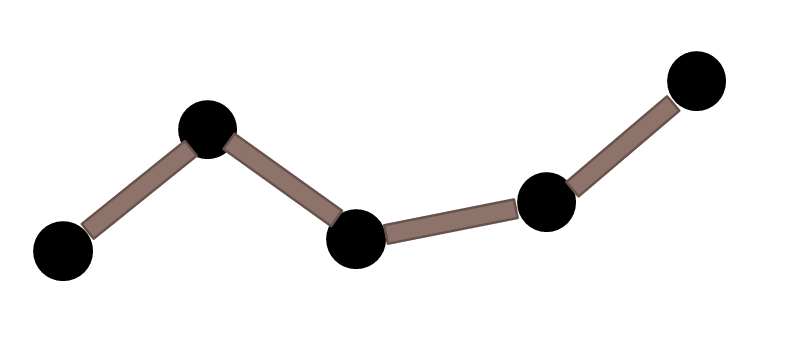
\includegraphics [scale=0.5] {my_folder/images//rope}
		\caption{Пример веревки. Черным обозначены частицы, коричневым обозначены ограничения}
		\label{fig:rope}  
	\end{figure}
	
	Проверим эмпирически, имеет ли место влияние порядка обхода на сходимость. Для этого поставим следующий эксперимент:
	\begin{itemize}
		\item Рассматривается одномерное пространство
		\item В данном пространстве помещается веревка, состоящая из четырёх частиц
		\item Крайняя левая частица оттягивается от остальных и закрепляется в пространстве
		\item Рассматривается работа первой итерации двух вариантов алгоритма PBD, обрабатывающих ограничения в разном порядке. Первый - слева направо, второй - справа налево.
	\end{itemize}
	
	\begin{figure}[ht!] 
		\center
		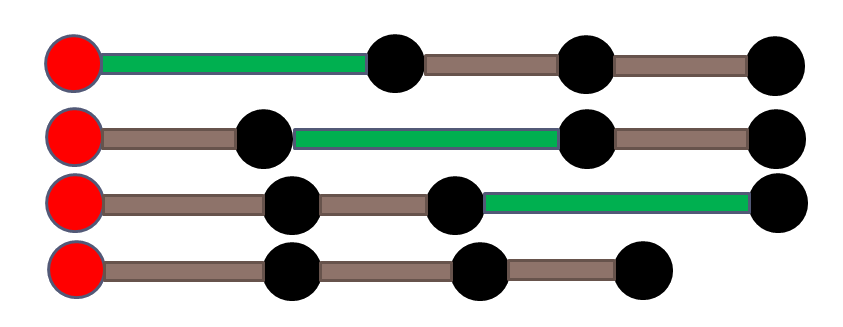
\includegraphics [scale=0.5] {my_folder/images//experiment_forward.png}
		\caption{Эксперимент с обходом слева направо. Сверху вниз представлены состояния веревки на каждом шаге первой итерации алгоритма PBD. Черным обозначены частицы, коричневым обозначены ограничения. Красным обозначена закрепленная частица, зеленым обозначено ограничение, которое будет обрабатываться следующим.}
		\label{fig:experiment-forward}  
	\end{figure}

	\begin{figure}[ht!] 
		\center
		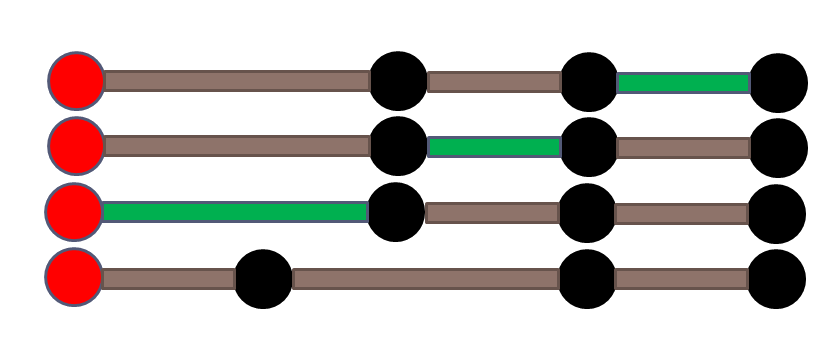
\includegraphics [scale=0.5] {my_folder/images//experiment_backward.png}
		\caption{Эксперимент с обходом справа налево. Сверху вниз представлены состояния веревки на каждом шаге первой итерации алгоритма PBD. Черным обозначены частицы, коричневым обозначены ограничения. Красным обозначена закрепленная частица, зеленым обозначено ограничение, которое будет обрабатываться следующим.}
		\label{fig:experiment-backward}  
	\end{figure}	
	
	Из экспериментов, продемонстрированных на \firef{fig:experiment-forward} и \firef{fig:experiment-backward}, можно заметить, что обход слева направо (\firef{fig:experiment-forward}) позволяет за первую итерацию перенести растяжение с первого ограниченичения до последнего и убрать его полностью за счет крайней правой вершины. С другой стороны, обход справа налево (\firef{fig:experiment-backward}) за первую итерацию перенес растяжение только на второе ограничение. Стоит отметить, что результаты данного эксперимента совпадает с результатами, полученными в \cite{gu2017constraint}.
	
	Однако, данный эксперимент показывет только влияние двух обходов, и только на первую итерацию алгоритма. В связи с этим, поставим следующий эксперимент:
	
	\begin{itemize}
		\item Рассматривается одномерное пространство.
		\item В данном пространстве помещается нерастяжимая веревка, состоящая из $N$ частиц.
		\item Каждая частицы находится на единичном расстоянии относительно соседних частиц.
		\item Для каждого ограничения расстояние покоя принимается равным единице.
		\item Крайняя левая частица оттягивается от остальных частиц и закрепляется в пространстве таким образом, чтобы расстояние между ней и соседней частицей стало равно двум.
		\item Рассматриваются следующие порядки обхода
			\begin{enumerate}[1.]
				\item $forward$ - обход слева направо.
				\item $backward$ - обход справа налево.
				\item $shuffle$ - каждая четная итерация запускается по обходу слева направо, каждая нечетная итерация запускается по обходу справа налево.
				\item $random$ - на каждой итерации список ограничений перемешивается и обрабатывается в случайном порядке.
				\item $coloring$ - сначала обрабатываются ограничения с четными номерами, затем ограничения с нечетными номерами.
			\end{enumerate}
		\item Запускается алгоритм PBD с различными наборами параметров, и подсчитывается, сколько итераций потребовалось, для того чтобы веревка была просимулирована
		\item Веревка считается просимулированной, если сумма модулей значений функций ограничений стала меньше значения погрешности, принятого равным $10^{-5}$
	\end{itemize}
	
	Данный эксперимент был поставлен с использованием языка программирования Python. Результаты данного эксперимента приведены в \taref{tab:order-experiment}.
	
	\noindent % for correct centering
	\begin{minipage}{\textwidth}
		\vspace{\mfloatsep} % интервал 
		\centering\small
		\captionof{table}{Результаты эксперимента применения различных обходов для различных веревок в одномерном пространстве}%
		\label{tab:order-experiment}
		\begin{tabular}{|l|l|c|}
			\hline
			\textbf{N} & \textbf{Порядок обхода} & \textbf{Количество итераций} \\
			\hline
			$4$ & $forward$ & $41$  \\ \hline
			$4$ & $backward$ & $43$ \\ \hline
			$4$ & $shuffle$ & $63$  \\ \hline
			$4$ & $random$ & $51$   \\ \hline
			$4$ & $coloring$ & $42$ \\ \hline
			$8$ & $forward$ & $229$  \\ \hline
			$8$ & $backward$ & $235$ \\ \hline
			$8$ & $shuffle$ & $278$  \\ \hline
			$8$ & $random$ & $293$   \\ \hline
			$8$ & $coloring$ & $232$ \\ \hline
			$16$ & $forward$ & $1064$  \\ \hline
			$16$ & $backward$ & $1078$ \\ \hline
			$16$ & $shuffle$ & $1156$  \\ \hline
			$16$ & $random$ & $1353$   \\ \hline
			$16$ & $coloring$ & $1071$ \\ \hline
			$32$ & $forward$ & $4562$  \\ \hline
			$32$ & $backward$ & $4592$ \\ \hline
			$32$ & $shuffle$ & $4738$  \\ \hline
			$32$ & $random$ & $5749$   \\ \hline
			$32$ & $coloring$ & $4577$ \\ \hline
			$64$ & $forward$ & $18876$  \\ \hline
			$64$ & $backward$ & $18938$ \\ \hline
			$64$ & $shuffle$ & $19222$  \\ \hline
			$64$ & $random$ & $23746$   \\ \hline
			$64$ & $coloring$ & $18907$ \\ \hline	
		\end{tabular}
		\vspace{\mfloatsep} % интервал 
		\normalsize %восстанавливаем шрифт 	
	\end{minipage}
	
	На основании полученных данных можно сделать следующие выводы:
	\begin{enumerate}[1.]
		\item Порядок обхода влияет на количество итераций
		\item Количество частиц в верёвке влияет на количество итераций
		\item Наблюдается квадратичная зависимость количества итераций от количества частиц
		\item Порядок обхода влияет на количество итераций много меньше, чем количество частиц
		\item Наилучшим с точки зрения количества итераций является обход $forward$, что соответствует наблюдению в работе \cite{gu2017constraint}
		\item Вторым по количеству итераций является обход $coloring$
	\end{enumerate}
	
	Стоит отметить, что обход $forward$, несмотря на то, что является оптимальным по количеству итераций, не применим в параллельной реалиазации. В свою очередь, обход $coloring$, основанный на принципе реберной раскраски графа, может быть применён в параллельном алгоритме, так как, в силу определения реберной раскраски, никакие два ребра одного цвета не имеют общих вершин. Это означает, что можно параллельно обрабатывать все ограничения, соответствующие ребрам одного цвета, тем самым уменьшив время выполнения одной итерации. 

%% Вспомогательные команды - Additional commands
%
%\newpage % принудительное начало с новой страницы, использовать только в конце раздела
%\clearpage % осуществляется пакетом <<placeins>> в пределах секций
%\newpage\leavevmode\thispagestyle{empty}\newpage % 100 % начало новой страницы